
Emacs 是一个强大的集成开发环境,
我们可利用它写代码、编译、调试、写文档,
我们甚至可以利用它上网,浏览网页,看视频,收发邮件等,
使用它可以极大地提高我们的工作效率。
学习 Emacs 的关键在于牢记各种快捷键,
减少在键盘和鼠标间的切换。
对于初学者建议按如下步骤学习 Emacs:
\begin{itemize}
	\item 阅读 Emacs Tutorial(进入 Emacs 后使用快捷键 Ctrl-h t)。
		其主要介绍基本的文本查看,编辑和查找操作,
		目的是让初学者对 Emacs 有一个大体的认识。
	\item 如果你想更加深入的了解Emacs,可以阅读书籍 
		Learning GNU Emacs\cite{cameron1996learning}, 
		这里推荐阅读 Chapter 5,8,9。
	\item 此时的你已能解决大多数问题,若还想继续学习 Emacs 的高级功能,
		可以学习 Emacs Lisp 语言,
		参考书籍 An Introduction to Programming in Emacs Lisp
		\cite{chassell2004introduction}。
\end{itemize}
在这里我们不过多介绍 Emacs 中的快捷键,
因为你可以在阅读上面书籍的过程中频繁遇到。
Emacs是绝对值得投入时间和经历的,因为你的回报会远远高出投入。



\subsection{Emacs + AUCTeX}

Emacs + AUCTeX 是一个能极大限度提高 \LaTeX 编辑效率的编辑器。
这是因为其具有强大的快捷键系统,方便的自动补全,
完善的引用系统以及快捷的自定义模板与环境等等。
当然效率的提高程度取决于你对它们的熟悉程度,不要因为刚入手时的困境而放弃。
这里我们简单的介绍一下其使用方法


\begin{itemize}	
	\item \textbf{安装:}可以在终端输入以下命令
	\begin{verbatim}
	sudo apt-get install emacs texlive-full auctex latex-cjk-*
	\end{verbatim}
    当然也可使用 Synaptic Package Manager 进行上述软件的安装。

	\item \textbf{核心操作:}
	\begin{itemize}
  		\item 打开一个文件(C-x C-f + 文件名),该命令后总是跟随这目录/文件名的,
  			如果要打开的文件不存在,就创建新文件;
  		\item 保存文件(C-x C-s),退出Emacs(C-x C-c);
  		\item 编译文档(C-c C-c),预览(C-c C-v),编译文档并查看(C-c C-a)。 
	\end{itemize}

	\item \textbf{基本操作:}
	\begin{itemize}
		\item 插入环境:通过 C-c C-e + 环境类型 命令添加环境
			\begin{verbatim}
			\begin{环境类型}
			\end{环境类型}
			\end{verbatim}
			可以使用 TAB 键查看环境类型列表或者自动补全;
		\item 插入宏:通过 C-c + Enter 命令插入宏,
			接着输入命令名称(usepackage,doucument 等等),
			最后选择输入命令的参数(没有可直接回车)。
			如果需要,你也可以添加相应的标签(可选),
			同样可以使用 TAB 键查看宏类型列表或者自动补全; 
		\item 快速更改字体(这系列命令一致以 C-c C-f 为前缀),如
			\begin{verbatim}
			C-c C-f C-e  // 插入强调字体 \emph{};
			\end{verbatim}
		\item 插入各级标题:通过 C-c C-s 命令插入标题,
			接着输入章节层级(section,subsection 等等),
	    	最后输入标题内容即可;
		\item 进入数学环境:通过 C-c $\sim$ 命令进入数学环境,
			里面快捷键很多,可以在菜单栏查看;
		\item 选择,注释,编译片段文件:
			\begin{verbatim}
			C-c C-r  编译区域
			C-c ;    注释/取消注释区域
			\end{verbatim}
		\item Emacs 内预览(在 Preview 菜单栏内查看);
		\item 多文件管理。
			编写较大的文档时,
			通常会使用 include 或 input 命令将主要章节分离成独立的文件。
			这时就需要在编写子文件的时候,键入编译和预览命令时,
			AUCTeX 能主动定位主文档并执行命令。
			为了做成这件事,需要首先在 .emacs 中添加命令
			\begin{verbatim}
			;; Query for master file.
			(setq-default Tex-master nil)
			\end{verbatim}
			之后,在每次创建新文件的时候我们都需要指定该文件的主文件,
			其基本命令为
			\begin{verbatim}
			C-c _ 
			\end{verbatim}
			然后输入主文件路径信息即可(不显示指明路径即默认该文件为主文件)。
			在编辑子文件时,输入
			\begin{verbatim}
			C-c ^
			\end{verbatim}
			即可返回到主文件。
			在子文件输入编译或者预览命令即可实现全局编译与预览。
	\end{itemize}
\end{itemize}

值得注意的是,使用 AUCTeX 前你不得不学会一些 \LaTeX 的基本句法。
不过作为一个刚接触 \LaTeX 或者接触 \LaTeX 不久的初学者,
设计一个精美的文档是相对困难的,
这时可以适当参考一些优秀的模板(如,\url{http://www.latextemplates.com})。
利用这些模板,我们可以轻松的表达我们想写的内容而不是注重文档设计的形式。
但无论什么时候,都要记住一个原则,即\textbf{保持源码的简洁性}。
大至整个文档的设计,小到每个语法,
其目的是为了方便阅读或者修改。

对于一个科研工作者来说,仅仅会用 \LaTeX 写文档是远远不够的。
在学习的生涯中,你可能会有无数次的报告,展示,答辩等等。
相比于传统的 PPT 展示,
利用 beamer 制作学术讲稿更加方便,美观。
因为其兼容 \LaTeX 命令,对于现有文章中的定义、定理、公式、算法、代码、图表等复杂内容,
只需要简单粘贴到 beamer 里面直接使用即可。
并且其输出为 PDF,具有很强的可读性,跨平台显示也无差异。
下面是一个简单的例子(其效果图见 \ref{fig:beamer}):
\begin{verbatim}
%!TEX program = xelatex

\documentclass{beamer}
\usepackage{xeCJK}

% 使用的主题,Beamer 因为有各种主题才使得有生气
\usetheme{Madrid}

\title[简短的标题]{这是一个简单的 \LaTeX 展示}
\author[作者]{xxx}
\institute[作者机构]{作者机构/信息}
\date[\today]{\today}

\begin{document}

% 标题页帧
\frame{\titlepage}
% 普通帧
\begin{frame}\frametitle{标题}
  这里是需要表达的内容!通常包括基本的文本,表格,图片等等!
\end{frame}

\end{document}
\end{verbatim}

\begin{figure}[htbp]
	\centering
	\subfigure[标题页帧]{
		
\includegraphics[width=0.48\linewidth]{png/beamer1}
	}
	\hfill
	\subfigure[普通帧]{
		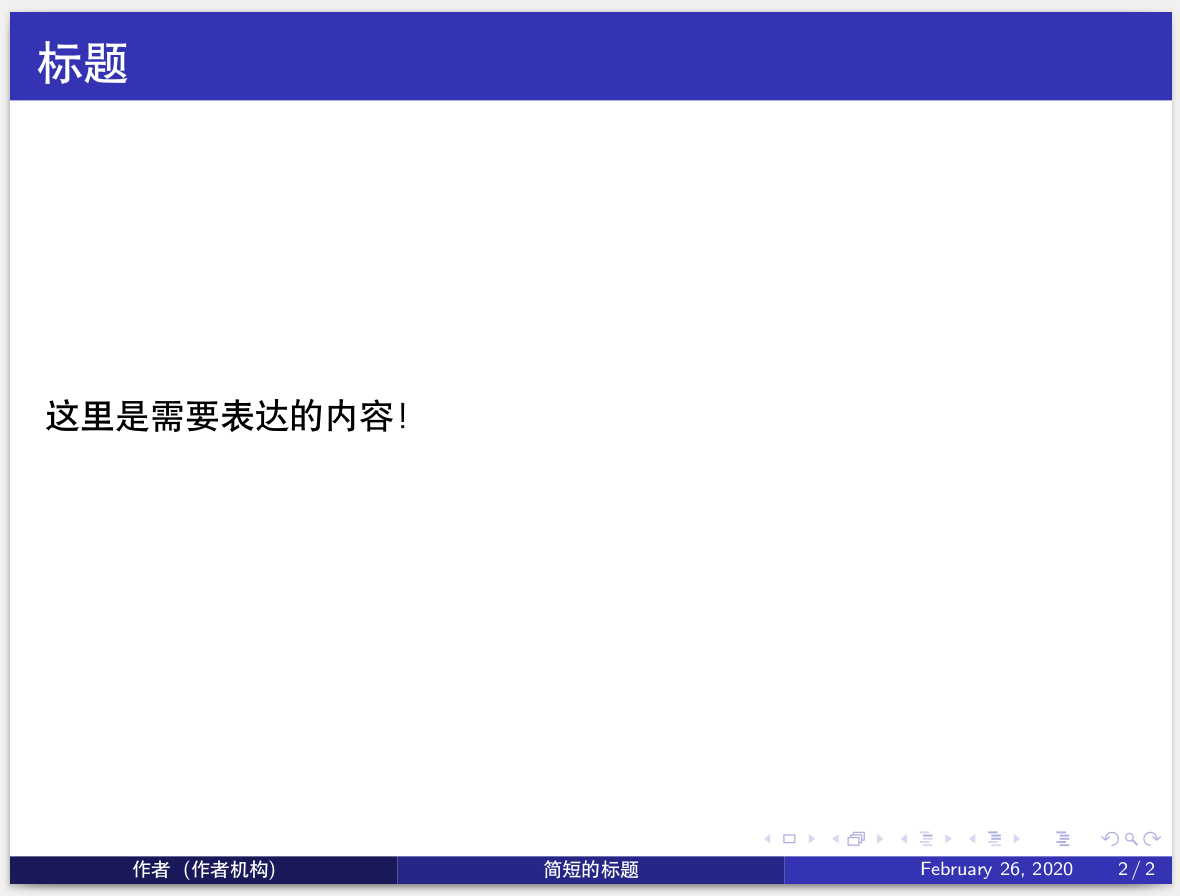
\includegraphics[width=0.48\linewidth]{png/beamer2}
	}
        \caption{标题和普通帧。}
	\label{fig:beamer}
\end{figure}

这里我们看到的每一页 PDF 即是所谓幻灯片的帧(frame),
Beamer 的帧分为两类,即
\begin{itemize}
	\item 标题页帧,语法为:
	\begin{verbatim}
	\frame{\titlepage}
	\end{verbatim}
	在这上面,一般会有标题、作者、时间、机构,LOGO等信息。
	\item 普通帧,主要为需要展示的内容,基本语法为:
	\begin{verbatim}
	\begin{frame}\frametitle{标题}
  	这里是需要表达的内容!
	\end{frame}
	\end{verbatim}
\end{itemize}

最后我们简要介绍一下 \LaTeX 中的作图工具---PSTricks。
它是一个基于 PS 的宏包,有了它我们就可以直接在 \LaTeX 文档中绘制非常复杂的图形。
但其命令繁琐,不太直观,所以不易熟练掌握。
初期,我们需要知道其基本语法,并学会绘制简单的图形。

\begin{itemize}
	
	\item 基本语法(因为 \LaTeX 绘图指令功能很弱,对较复杂的图形无能为力,
	一般都是用绘图软件事先将图形绘制好,再用图形输入命令插入 \LaTeX 源文件中,
	每一个图形的语法一般如下):
	\begin{verbatim}
	\documentclass[10pt]{article}

	\usepackage{amsmath}
	\usepackage{pstricks,pst-eps}
	\pagestyle{empty}

	\begin{document}
  	  \begin{TeXtoEPS}
    	\begin{pspicture}(5.5,5.5)

      	% Triangle in red:
      	\pspolygon[linecolor=red](1,1)(5,1)(1,4)
      	% Bezier curve in green:
      	\pscurve[linecolor=green,linewidth=2pt,%
      	showpoints=true](5,5)(3,2)(4,4)(2,3)
     	% Circle in blue with radius 1:
      	\pscircle[linecolor=blue,linestyle=dashed](3,2.5){1}

    	\end{pspicture}
  	  \end{TeXtoEPS}
	\end{document}
	\end{verbatim}
	其中紧跟在 pspicture 环境后面的 $(x_0,y_0), (x_1,y_1)$ 参数表示所绘制图形的大小,
	这个图形左下角的坐标在 $(x_0,y_0)$(不显示指明默认为原点),
	右上角的坐标在 $(x_1,y_1)$,生成的图形不能越过这个长方形的范围。
	每一个基本命令包括图形对象和图形参数。
	简单的如点、 线段,复杂的如各种曲线或自定义的图形都被称为图形对象。
	一个图形对象对应着一条命令, 一般的形式是
	\begin{verbatim}
	命令 [选项] ... 
	\end{verbatim}	
	其中选项可以是一个,也可以有多个,多个选项之间用逗号分隔。
	选项中一般设置绘制对象时的线条、颜色属性,这些属性又被称为图形参数。
	详细命令可以参考书籍
	PSTricks : PostScript macros for Generic TeX \cite{van1993pstricks}。
	\item Makefile 文件(负责由源代码生成 eps 格式图片):
	\begin{verbatim}
	allEps : test.eps
	clean :
   		rm *.aux *.log *.cache
	%.eps : %.dvi
   		dvips $< -E -o $@
	%.dvi : %.tex
   		latex $<
	\end{verbatim}
\end{itemize}

最后只需要在终端输入 make,
即可以得到我们想要绘制的图形(见 \ref{fig:pstricks})。

\begin{figure}[htbp]
	\centering
	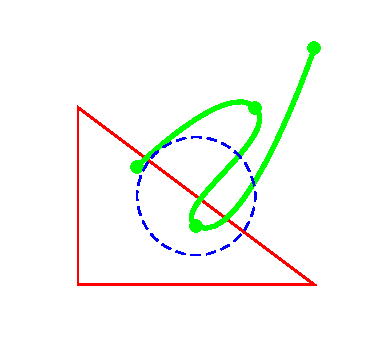
\includegraphics[width=0.4\textwidth]{eps/pstricks}
	\caption{使用 PSTricks 绘制的图片。}
	\label{fig:pstricks}
\end{figure}


